%% Le lingue utilizzate, che verranno passate come opzioni al pacchetto babel. Come sempre, l'ultima indicata sarà quella primaria.
%% Se si utilizzano una o più lingue diverse da "italian" o "english", leggere le istruzioni in fondo.
\def\thudbabelopt{english,italian}
%% Valori ammessi per target: bach (tesi triennale), mst (tesi magistrale), phd (tesi di dottorato).
%% Valori ammessi per aauheader: '' (vuoto -> nessun header Alpen Adria Univeristat), aics (Department of Artificial Intelligence and Cybersecurity), informatics (Department of Informatics Systems). Il nome del dipartimento è allineato con la versione inglese del logo UniUD.
%% Valori ammessi per style: '' (vuoto -> stile moderno), old (stile tradizionale).
\documentclass[target=bach,aauheader=,style=]{thud}

%% --- Informazioni sulla tesi ---
%% Per tutti i tipi di tesi
% Scommentare quello di interesse, o mettete quello che vi pare
\course{Informatica}
%\course{Internet of Things, Big Data e Web}
%\course{Matematica}
%\course{Comunicazione Multimediale e Tecnologie dell'Informazione}
\title{RAM-USB \\Progettazione e implementazione \\ di un server di backup multi utente \\ Zero-Knowledge e Zero-Trust  \\ }
\author{Francesco Verrengia}
\supervisor{Prof.\ Ivan Scagnetto}
\cosupervisor{}
\tutor{}
%% Campi obbligatori: \title, \author e \course.
%% Altri campi disponibili: \reviewer, \tutor, \chair, \date (anno accademico, calcolato in automatico), \rights
%% Con \supervisor, \cosupervisor, \reviewer e \tutor si possono indicare più nomi separati da \and.
%% Per le sole tesi di dottorato:
\phdnumber{313}
\cycle{XXVIII}
\contacts{Via della Sintassi Astratta, 0/1\\65536 Gigatera --- Italia\\+39 0123 456789\\\texttt{http://www.example.com}\\\texttt{inbox@example.com}}

%% --- Pacchetti consigliati ---
%% pdfx: per generare il PDF/A per l'archiviazione. Necessario solo per la versione finale
\usepackage[a-1b]{pdfx}
%% hyperref: Regola le impostazioni della creazione del PDF... più tante altre cose. Ricordarsi di usare l'opzione pdfa.
\usepackage[pdfa]{hyperref}
\usepackage{float}
%% float: gli schemi di flusso crittografico non sono figure né tabelle, quindi hanno un proprio
%% tipo di float, numerato per capitolo come gli altri. \floatname fissa la parola che compare
%% nella didascalia, \schemaautorefname quella che \autoref stampa nel testo.
\newfloat{schema}{H}{los}[chapter]
\floatname{schema}{Schema}
\providecommand{\schemaautorefname}{Schema}
\usepackage{longtable}
%% enumitem: la classe thud applica setstretch{1.3} a tutto il corpo, che gonfia anche la
%% spaziatura di default di itemize/enumerate. Questi valori la riportano a qualcosa di leggibile.
\usepackage{enumitem}
\setlist{itemsep=2pt, topsep=4pt, parsep=0pt, partopsep=0pt}
%% La classe book, in modalità twoside (usata da thud.cls), usa flushbottom di default: LaTeX
%% allunga gli spazi elastici (dopo i \section, tra i paragrafi, prima delle liste) per far
%% arrivare il testo esattamente al margine inferiore, anche quando la pagina ha poco contenuto —
%% è la vera causa dei grandi vuoti "a caso" osservati. raggedbottom lo disattiva.
\raggedbottom
%% Margine di sicurezza per righe che altrimenti andrebbero overfull (es. un \item in grassetto
%% seguito da un lungo elenco di nomi propri, senza molti punti di interruzione naturali).
\setlength{\emergencystretch}{2em}
\hypersetup{hidelinks}
%% listings: frammenti di codice Go copiati verbatim dai sorgenti del progetto. Il linguaggio Go
%% non è tra quelli predefiniti del pacchetto, quindi va dichiarato qui.
\usepackage{listings}
\lstdefinelanguage{Go}{
  morekeywords={break,case,chan,const,continue,default,defer,else,fallthrough,for,func,go,goto,%
    if,import,interface,map,package,range,return,select,struct,switch,type,var,nil,true,false,%
    make,new,len,cap,append,copy,error,string,byte,rune,bool,int,int64,uint8,uint32},
  sensitive=true,
  morecomment=[l]{//},
  morecomment=[s]{/*}{*/},
  morestring=[b]",
}
%% Le direttive di sshd_config non sono un linguaggio predefinito di listings: dichiararle qui fa
%% si che i frammenti di configurazione siano evidenziati come quelli di codice, invece di restare
%% monospazio piatto.
\lstdefinelanguage{sshdconfig}{
  morekeywords={AllowAgentForwarding,AllowTcpForwarding,AllowUsers,AuthorizedKeysCommand,%
    AuthorizedKeysCommandUser,AuthorizedKeysFile,ChrootDirectory,Ciphers,ForceCommand,HostKey,%
    HostKeyAlgorithms,KbdInteractiveAuthentication,KexAlgorithms,ListenAddress,LoginGraceTime,%
    MACs,Match,MaxAuthTries,MaxSessions,MaxStartups,PasswordAuthentication,PermitEmptyPasswords,%
    PermitRootLogin,PermitTunnel,PermitUserRC,Port,PubkeyAuthentication,Subsystem,User,UsePAM,%
    X11Forwarding},
  %% Senza questo, listings spezza gli identificatori sulle cifre e X11Forwarding resterebbe
  %% l'unica direttiva non evidenziata del listato.
  alsoletter=0123456789,
  morecomment=[l]{\#},
  sensitive=true,
}
%% Lo schema SQL della tabella dei grant (cap. 7) non è nemmeno lui un linguaggio predefinito di
%% listings: stessa ragione del blocco sshdconfig sopra.
\lstdefinelanguage{sql}{
  morekeywords={CREATE,TABLE,IF,NOT,EXISTS,PRIMARY,KEY,NULL,DEFAULT,UNIQUE,REFERENCES,%
    INTEGER,TEXT,REAL,BLOB,SELECT,INSERT,INTO,VALUES,WHERE,UPDATE,DELETE,FROM,AND,OR,%
    ALTER,SET,CALL},
  sensitive=false,
  morecomment=[l]{--},
  morestring=[b]',
}
%% Palette dei listati: il colore affianca grassetto e corsivo, non li sostituisce, cosi il
%% codice resta leggibile anche stampato in bianco e nero.
\definecolor{lstkeyword}{RGB}{0,70,140}
\definecolor{lstcomment}{RGB}{100,100,100}
\definecolor{lststring}{RGB}{0,110,70}
\definecolor{lstrule}{RGB}{120,120,120}
\lstset{
  language=Go,
  basicstyle=\ttfamily\footnotesize,
  keywordstyle=\bfseries\color{lstkeyword},
  commentstyle=\itshape\color{lstcomment},
  stringstyle=\color{lststring},
  columns=fullflexible,
  breaklines=true,
  breakatwhitespace=true,
  showstringspaces=false,
  tabsize=4,
  captionpos=b,
  xleftmargin=1em,
  rulecolor=\color{lstrule},
  frame=tb,
  framerule=0.5pt,
  framesep=6pt,
  aboveskip=1.2em,
  belowskip=0.8em,
}
\renewcommand{\lstlistingname}{Codice}
\providecommand{\lstlistingautorefname}{Codice}
%% needspace: evita che un frammento di codice venga spezzato tra due pagine.
\usepackage{needspace}
%% tocbibind: Inserisce nell'indice anche la lista delle figure, la bibliografia, ecc.

%% --- Stili di pagina disponibili (comando \pagestyle) ---
%% sfbig (predefinito): Apertura delle parti e dei capitoli col numero grande; titoli delle parti e dei capitoli e intestazioni di pagina in sans serif.
%% big: Come "sfbig", solo serif.
%% plain: Apertura delle parti e dei capitoli tradizionali di LaTeX; intestazioni di pagina come "big".

%% Se il file no-dedica.flag esiste in questa cartella, la dedica viene omessa dalla compilazione.
%% Creato/rimosso dai target 'thesis'/'thesis-no-dedica' del Makefile in radice — non va creato/rimosso
%% a mano, e non deve restare presente dopo una compilazione manuale con pdflatex/latexmk.
\newif\ifNoDedica
\IfFileExists{no-dedica.flag}{\NoDedicatrue}{\NoDedicafalse}

\begin{document}
\maketitle

%% Dedica (opzionale) — omessa se no-dedica.flag esiste (vedi sopra)
\ifNoDedica\else
\input{chapters/00_dedica}
\fi

%% Ringraziamenti (opzionali) — omessi se no-dedica.flag esiste (vedi sopra)
\ifNoDedica\else
\input{chapters/00_ringraziamenti}
\fi

%% Sommario (opzionale), capitolo a parte
\abstract
RAM-USB è un servizio di backup multi-utente, geo-distribuito e accessibile da remoto, progettato
secondo tre principi di sicurezza: zero-knowledge, nessun componente lato server accede mai al
contenuto dei backup in chiaro; zero-trust, nessun componente si fida implicitamente dei dati ricevuti
da un altro; defense-in-depth, ogni strato rivalida indipendentemente l'input ricevuto. Il progetto nasce 
come caso di studio approfondito sulla progettazione di sistemi di backup distribuiti.

Il sistema è un'architettura a microservizi n-tier: ogni registrazione o login attraversa quattro
processi distinti, ciascuno dei quali rivalida l'input senza fidarsi dello strato precedente, mentre
l'accesso allo spazio di backup, isolato per utente tramite chroot dinamico, resta possibile solo dopo
l'autenticazione, su una rete privata mesh che applica confini di raggiungibilità distinti per ogni fase
del ciclo di vita dell'utente. I requisiti sono raccolti in un unico documento tracciabile fino al
codice, con un modello a spirale per l'analisi e un modello a V per l'implementazione.

L'analisi critica delle proprietà di sicurezza quantifica il costo di un attacco offline alle password,
giorni per la lunghezza minima ammessa, ordini di grandezza superiori per password più lunghe, e
verifica componente per componente che la compromissione isolata di un servizio non si propaghi agli
altri. Ogni scelta architetturale è messa a bilancio con il prezzo che comporta, dalla latenza
introdotta dalla separazione in più processi alla complessità della rivalidazione indipendente.

Il sistema è stato distribuito e verificato end-to-end su un'infrastruttura reale. 
I suoi limiti del sisitema sono dichiarati insieme agli sviluppi che potrebbero mitigarli.


%% Indice
\tableofcontents

%% Lista delle tabelle (se presenti)
%\listoftables

%% Lista delle figure (se presenti)
%\listoffigures

%% Corpo principale del documento
\mainmatter

%% Parte
%% La suddivisione in parti è opzionale; solitamente sono sufficienti i capitoli.
%\part{Parte}

%% Capitoli: un file per capitolo sotto chapters/, richiamato con \input.
%% Per aggiungere un nuovo capitolo: crea chapters/NN_nome.tex e aggiungi un \input qui sotto.
\chapter{Introduzione}
\label{chap:introduzione}

\section{Contesto}

Un backup, nell'ambito della sicurezza informatica, è un processo di disaster recovery: un procedimento
che consente di recuperare dati andati persi, per esempio in seguito a un attacco, un guasto hardware o
software, o un errore umano. Una delle prime risposte tecniche alla perdita di dati è la ridondanza dei dischi su
cui questi sono memorizzati: nel 1988 Patterson, Gibson e Katz formalizzano il RAID (Redundant Array of
Inexpensive Disks), che distribuisce lo stesso dato su più dischi economici per ottenere un'affidabilità
paragonabile a quella di un singolo disco più costoso \cite{patterson-gibson-katz-raid-1988}.

Questa ridondanza, però, resta locale e non protegge da un evento che distrugga l'intero apparato. Da
qui nasce l'esigenza di un backup remoto: una copia dei dati conservata in un luogo diverso da quello
degli originali. Il modo più semplice è affidarli a terzi, un conoscente che possiede l'hardware o
un'attività commerciale che offre questo tipo di servizio, ma questo richiede di fidarsi che quei dati
non vengano letti, modificati o venduti da chi li conserva.

Chi offre il servizio, dal canto suo, trova conveniente servire più utenti contemporaneamente. Questo
richiede però di distinguere gli utenti, e di garantire che ciascuno acceda solo ai propri dati: in
pratica, richiede un sistema di autenticazione e controllo degli accessi.

Tra i diversi sistemi di autenticazione esistenti, quello adottato e discusso in questa tesi è basato su 
email e password che, in quanto dati sensibili, richiedono un livello di protezione elevata. 
Il principio su cui si fonda questo tipo di autenticazione è semplice:
l'utente si registra inviando al server le proprie credenziali; durante il login le invia di nuovo, e il
server le confronta con quelle salvate in fase di registrazione. Se coincidono, l'utente è autenticato.

Il fatto che il server possieda le credenziali espone quindi tutti gli utenti al rischio che vengano
rubate. Esistono numerosi sistemi per impedirlo; uno tra tutti, approfondito in questa tesi, è l'uso di
una funzione di hash.
Il server, al posto di salvare le credenziali in chiaro, le salva
sotto forma di hash. Durante il login, ricalcola gli hash delle credenziali fornite dall'utente e
verifica se coincidono con quelli salvati.

\subsection{Funzioni di hash}

Le funzioni di hash sono funzioni non invertibili che trasformano un input di lunghezza
arbitraria in un output di lunghezza fissa e strettamente correlato con i dati di input, chiamato hash.
Indicata con $H$ una funzione di hash, questa gode delle seguenti proprietà fondamentali:

\begin{itemize}
    \item \textbf{resistenza alla preimmagine:} dato $h$, è computazionalmente intrattabile trovare $x$
    tale che $H(x) = h$;
    \item \textbf{resistenza alla seconda preimmagine:} data $x$, è computazionalmente intrattabile
    trovare $y \neq x$ tale che $H(x) = H(y)$;
    \item \textbf{resistenza alle collisioni:} è computazionalmente intrattabile trovare una coppia
    $(x, y)$ con $x \neq y$ tale che $H(x) = H(y)$.
\end{itemize}


\section{Problema affrontato}

Tra le cause di perdita dei dati elencate sopra, RAM-USB si concentra sull'attacco da parte di un 
malintenzionato, affidandosi ai principi zero-trust e defense-in-depth nel tentativo di garantire la 
sicurezza dei dati anche quando un componente qualsiasi del sistema viene compromesso.

\section{Obiettivi}

RAM-USB, Remotely Accessible Multi-User Secure Backup è un caso di studio approfondito sulla progettazione, 
implementazione e distribuzione di un servizio di backup che soddisfi i requisiti
descritti nel \autoref{chap:requisiti}. Non è pensato per competere con le soluzioni 
commerciali esistenti, ma per discuterne le scelte di design, illustrandone pro e contro in modo 
trasparente, con un approccio security first e concentrato sulla difesa del sistema da attacchi esterni.


\section{Metodologia}
Parte dei componenti di RAM-USB nascono dalla fase di brainstorming condotta insieme a Riccardo 
Gottardi \cite{gottardi-github}.

La metodologia adottata combina il modello a spirale per la definizione e l'evoluzione dei 
requisiti \cite{Boehm88} con l'approccio Test-Driven Development per l'implementazione e il modello a V per 
la loro verifica \cite{ramusb-contributing}.

Il linguaggio usato per l'intero stack è Go, un linguaggio compilato progettato esplicitamente per gestire 
in modo efficiente molte connessioni di rete simultanee.

Per orchestrare l'infrastruttura attorno al codice Go (avvio dei servizi, supervisione dei processi nei 
container, sequenziamento all'avvio) è stato usato il linguaggio Bash. 

Il codice è versionato con Git e pubblicato gratuitamente, in versione integrale su GitHub, distribuito con 
licenza MIT. 

L'implementazione è stata interamente realizzata con l'assistenza dei Large Language Model Claude 
Sonnet 4.5 e Sonnet 5, in forma multi-agentica tramite l'harness Claude Code eseguito in una macchina 
virtuale su Proxmox per questioni di sicurezza e privacy.

L'intelligenza artificiale generativa è stata impiegata esclusivamente come strumento sotto stretta 
supervisione umana. 
La progettazione, la struttura del codice, i confini dei moduli, la firma, il comportamento delle singole 
funzioni, e i test corrispondenti restano una decisione umana; l'assistente ha implementato solo quanto 
specificato, in passi piccoli, incrementali e verificabili, prendendosi la libertà implementativa di basso 
livello.
Ogni modifica è stata revisionata ed esplicitamente approvata prima di essere introdotta nella codebase.
Le numerose strategie di mitigazione degli errori implementativi e allucinazioni dei due modelli, nonchè la 
getione dei multipli agenti utilizzati non sono oggetto di questa tesi. 

\section{Struttura della tesi}

Il \autoref{chap:principi-fondanti} approfondisce i due principi di sicurezza su cui RAM-USB è costruito,
zero-trust e defense-in-depth, dalle loro origini alla loro applicazione all'informatica.

Il \autoref{chap:requisiti} descrive la metodologia con cui i requisiti sono stati raccolti e tracciati,
e i casi d'uso che ne derivano.

Il \autoref{chap:architettura} presenta i componenti che partecipano alla registrazione e al login.

Il \autoref{chap:autenticazione} segue le credenziali lungo quel percorso, dal confine pubblico fino al
record salvato, e descrive le regole che ogni strato applica.

Il \autoref{chap:storage} segue il backup fino al proprio spazio isolato su Storage-Service.

Il \autoref{chap:rete} descrive come la rete mesh applichi i confini di raggiungibilità tra i
componenti.

Il \autoref{chap:osservabilita} chiude il ciclo di vita di una richiesta con la pipeline di
osservabilità che la rende misurabile.

Il \autoref{chap:testing} verifica il sistema così costruito attraverso i quattro livelli del modello a
V, dal test di unità alla lista di accettazione, e riporta cosa ha trovato eseguendolo su hardware reale.

Il \autoref{chap:deployment} descrive come questi componenti siano effettivamente distribuiti, tra
container Docker, macchine Proxmox e un VPS pubblico.

Il \autoref{chap:sicurezza} rilegge l'intero sistema dal punto di vista di chi tenta di comprometterlo,
verificando quali garanzie resistano anche alla sua compromissione totale.

Il \autoref{chap:conclusioni} chiude la tesi bilanciando i risultati ottenuti con i limiti riscontrati,
e indicando gli sviluppi futuri più rilevanti.

\chapter{Stato dell'arte e contesto tecnologico}

\section{Principi di sicurezza di riferimento}
%% TODO: NIST SP 800-207 (Zero Trust), distinzione zero-knowledge/zero-knowledge proof.

\section{Soluzioni di backup esistenti}
%% TODO: restic (usato lato client), Tarsnap, Borg/BorgBackup.

\section{Paralleli in altri domini a conoscenza zero}
%% TODO: password manager (Bitwarden) e cloud storage E2E (Tresorit) come paralleli.

\section{Reti mesh e zero-trust networking}
%% TODO: Tailscale/WireGuard, cosa offre una mesh VPN vs una VPN centralizzata.

\section{Posizionamento di RAM-USB}
%% TODO: cosa distingue il progetto (case study, non prodotto) e cosa riprende da queste soluzioni.

\chapter{Analisi dei requisiti}

\section{Metodologia dei requisiti}
%% TODO: modello a spirale della SRS, tracciabilità requisito-permalink di codice.

\section{Requisiti utente e casi d'uso}
%% TODO: i 10 RU e i 5 UC della SRS, trattabili per intero.

\section{Requisiti funzionali: pattern trasversali}
%% TODO: pattern ricorrenti (validazione ridondante, mTLS punto-a-punto, mapping errori) con esempi, non elenco esaustivo.

\section{Requisiti non funzionali e di dominio}
%% TODO: §5-6 della SRS, pochi punti, trattabili per intero.

\chapter{Architettura generale e trust zones}

\section{Overview architetturale}

RAM-USB è un'architettura a microservizi n-tier in cui ogni componente ha una responsabilità specifica. 
Questa separazione riduce il rischio che la compromissione di un componente comprometta l'intero sistema.

RAM-USB ha dieci componenti interni, organizzati in tre gruppi funzionali: 
\begin{itemize}
    \item \textbf{Accesso e registrazione}: Entry-Hub, Security-Switch, Database-Vault, Network-Manager, Certificate-Authority, Headscale.
    \item \textbf{Backup e restore}: Storage-Service.
    \item \textbf{Osservabilità}: Mosquitto, Metrics-Collector, Grafana.
\end{itemize}

La \autoref{fig:architecture-container} mostra questi dieci componenti e il protocollo con cui interagiscono.

\begin{figure}[H]
    \centering
    \includegraphics[width=0.75\textwidth]{figures/01-architecture-container.pdf}
    \caption{Diagramma dei container di RAM-USB.}
    \label{fig:architecture-container}
\end{figure}

\subsection{Entry-Hub}

Entry-Hub è il gateway pubblico del sistema, ovvero l'unico esposto a chiunque su internet. Per questo 
il sistema non gli concede fiducia implicita. Il suo processo gira quindi in un container distroless 
\cite{distroless-github}, seguendo il principio di riduzione dell'attack surface raccomandato da 
NIST SP 800-190 \cite{nist-sp-800-190}. 
Senza shell, infatti, la maggior parte delle vulnerabilità critiche note nei container non è sfruttabile 
\cite{wager2024distroless}

Entry-Hub espone tre endpoint HTTPS: \texttt{POST /api/health} e \texttt{POST /api/register} sono
raggiungibili da chiunque su internet, con certificato firmato dalla CA pubblica Let's Encrypt
\cite{aas2019letsencrypt}. \texttt{POST /api/login} usa lo stesso certificato, ma ha un listener separato,
raggiungibile solo da utenti con accesso alla rete privata di cui parleremo in dettaglio nel
\autoref{chap:rete}.

Quando riceve una richiesta, Entry-Hub valida il corpo JSON in due fasi: in decodifica, impone un
limite di dimensione e rifiuta qualunque campo non atteso nel payload; poi valida i singoli
campi email, password e, solo in fase di registrazione, la chiave SSH \cite{ramusb-code-eh-f-04}. Se una di
queste verifiche fallisce, risponde HTTP 400 senza specificare quale sia il problema e senza inoltrare la
richiesta agli strati più interni del sistema. Se la validazione riesce, inoltra la richiesta a
Security-Switch via mTLS verificando che il certificato ricevuto appartenga davvero a un Security-Switch.
Attende la risposta del Security-Switch e la rilancia al client.

\subsection{Security-Switch}

Security-Switch è lo smistatore di richieste del sistema. Si occupa di ricevere le richieste da Entry-Hub e 
contattare i servizi interni. In questo modo la responsabilità di comunicare con i gestori del database e 
della rete non è in mano al punto di ingresso del sistema. 

Accetta connessioni in ingresso solo da Entry-Hub, autenticato via mTLS e, visto che il sistema tratta 
tutti i componenti come non fidati, ri-valida l'input in modo indipendente. 
Lo scopo di questa rivalidazione è l'applicazione del principio di defence in depth \cite{nist-sp-800-207}.

Se la validazione riesce, inoltra la richiesta a Database-Vault via mTLS. 

Nel caso di una richiesta di registrazione, chiede al Network-Manager di creare l'identità del nuovo utente 
sulla rete mesh e la credenziale (pre-auth key) con cui il suo dispositivo potrà unirvisi. 

Nel caso di una richiesta di login, chiede al Network-Manager di concedere un accesso temporaneo di 12 ore 
per quell'utente verso Storage-Service. 
Solo quando l'utente avrà ottenuto l'accesso allo Storage-Service, potrà contattarlo e gestire i propri backup.


\subsection{Database-Vault}


\subsection{Storage-Service}

\subsection{Network-Manager}

\subsection{Certificate-Authority}

\subsection{Headscale}

\subsection{Mosquitto}

\subsection{Metrics-Collector}

\subsection{Grafana}

\section{Modello di comunicazione inter-servizio}

\section{Trust zones e confini di sicurezza}
\label{sec:trust-zones}

\chapter{Autenticazione e gestione delle identità}
\label{chap:autenticazione}

\section{Ciclo di vita della richiesta}
\label{sec:ciclo-richiesta}

Una richiesta di registrazione o di login attraversa tre servizi prima di diventare un record:
Entry-Hub, Security-Switch e Database-Vault. Tutti e tre applicano le stesse verifiche sull'input,
ognuno indipendentemente dagli altri.

La validazione avviene in due fasi. La prima riguarda il corpo della richiesta: il payload viene
letto fino a un limite di 2048 byte e rifiutato se lo supera, senza accumulare in memoria dati
controllati da chi ha inviato la richiesta, e il decoder JSON respinge qualunque campo inatteso.

La seconda fase riguarda i singoli campi \cite{ramusb-code-eh-f-04}. L'email deve essere un
indirizzo singolo e sintatticamente valido secondo RFC 5322 \cite{rfc5322}; la password deve essere
lunga tra 8 e 128 caratteri e usare almeno tre categorie tra minuscole, maiuscole, cifre e simboli.
In registrazione, inoltre, la chiave pubblica SSH deve essere ben formata.

Se una verifica fallisce, la risposta è HTTP 400 senza indicare quale controllo non sia passato, il
log registra il problema senza identificare l'utente, e la richiesta non prosegue verso l'interno. 
Il messaggio resta generico perché un errore dettagliato aiuterebbe un attaccante più di quanto aiuti un
utente in buona fede, che le stesse verifiche le ha già ricevute dal proprio client.

I tre servizi condividono la stessa libreria di validazione, quindi ripetere il controllo non
introduce diversità algoritmica, ma garantisce che nessun servizio dia per scontato che il
precedente abbia fatto il proprio lavoro. In questo modo, se a Database-Vault dovesse arrivare una
richiesta proveniente da un servizio compromesso, la validazione verrebbe fatta comunque.

Gli errori interni vengono infine tradotti in codici HTTP. La \autoref{tab:codici-http} riassume i codici 
che raggiungono l'utente, attribuendo ciascun codice a chi lo emette.

Entry-Hub costruisce soltanto gli errori che nascono da sé stesso: una validazione fallita e una
chiamata a Security-Switch andata male. Tutto il resto lo rilancia al client così come gli arriva
dall'interno, senza modificarlo. Per questo motivo, un 401 o un 409 raggiungono l'utente pur non
essendo mai prodotti da Entry-Hub.

\begin{table}[H]
\centering
\caption{Codici HTTP restituiti al client e loro significato nel sistema.}
\label{tab:codici-http}
\begin{tabular}{@{}l p{\dimexpr0.58\linewidth\relax} l@{}}
\hline
\textbf{Codice} & \textbf{Significato} & \textbf{Emesso da} \\
\hline
400 & Validazione fallita, senza indicare quale controllo non sia passato & entrambi \\
401 & Credenziali non valide, non specifica se email inesistente o password errata & Security-Switch \\
403 & Rifiuto esplicito di Network-Manager & Security-Switch \\
409 & Email o chiave SSH già registrate, non specifica quale delle due & Security-Switch \\
500 & Errore interno non altrimenti classificato & entrambi \\
502 & Servizio a valle irraggiungibile o con risposta inattesa & entrambi \\
503 & Chiamata a Security-Switch scaduta & Entry-Hub \\
504 & Chiamata a Database-Vault o Network-Manager scaduta & Security-Switch \\
\hline
\end{tabular}
\end{table}

Tra i codici che i due servizi costruiscono per conto proprio ci sono due differenze: 
la prima è il 403, che solo Security-Switch può emettere, perché è l'unico dei due a poter ricevere un 
rifiuto esplicito da un servizio interno. La seconda riguarda le chiamate scadute: Entry-Hub risponde 503, 
Security-Switch 504.

In tutti i casi il corpo della risposta è sanificato, e il dettaglio dell'errore resta nei log
interni.

\section{Cifratura e hashing delle credenziali}

Database-Vault tratta i dati che riceve in tre modi diversi:

\begin{itemize}
    \item la chiave SSH è pubblica, quindi non necessita di segretezza;
    \item l'email è insieme una chiave di ricerca e un dato personale da proteggere;
    \item la password non deve essere recuperabile, nemmeno da chi amministra il database.
\end{itemize}

L'email viene normalizzata in minuscolo e ridotta al proprio digest SHA-256, che diventa la chiave primaria 
del record. La normalizzazione garantisce che lo stesso indirizzo scritto con lettere diverse al login 
produca la stessa chiave della registrazione.
Questo hash è deterministico per necessità, perché deve permettere il lookup. Il limite fondamentale di 
questo approccio, insieme alla sua mitigazione, è discusso nel \autoref{chap:sicurezza}.

Accanto al digest che fa da chiave di ricerca, il record conserva una copia cifrata, così che 
l'indirizzo resti recuperabile. Da una master key e da un salt casuale di 16 byte, generato per quel record, 
viene derivata con HKDF-SHA256 \cite{rfc5869} una chiave dedicata, con cui l'email è cifrata in
AES-256-GCM \cite{nist-sp-800-38d} usando un nonce casuale di 12 byte. Salt, nonce e testo cifrato
vengono salvati nel record, mentre la chiave derivata viene azzerata appena il cifrario l'ha consumata.
Derivare una chiave per ogni record, invece di cifrare tutto con la master key, riduce la quantità
di dati protetti da una singola chiave.

\Needspace{22\baselineskip}
\begin{lstlisting}[caption={Derivazione della chiave per record in \texttt{newGCM}, da
\texttt{encryption.go} \cite{ramusb-code-hkdf-newgcm}.}, label={lst:hkdf}]
func newGCM(masterKey, salt []byte) (cipher.AEAD, error) {
	derivedKey := make([]byte, derivedKeySize)
	kdf := hkdf.New(sha256.New, masterKey, salt, []byte(hkdfInfo))
	if _, err := io.ReadFull(kdf, derivedKey); err != nil {
		return nil, fmt.Errorf("encryption: derive key: %w", err)
	}

	block, err := aes.NewCipher(derivedKey)
	for i := range derivedKey {
		derivedKey[i] = 0
	}
	if err != nil {
		return nil, fmt.Errorf("encryption: new AES cipher: %w", err)
	}

	gcm, err := cipher.NewGCM(block)
	if err != nil {
		return nil, fmt.Errorf("encryption: new GCM: %w", err)
	}

	return gcm, nil
}
\end{lstlisting}


La password viene invece concatenata a un pepper, letto da una variabile d'ambiente, e passata ad Argon2id 
\cite{rfc9106} insieme a un salt casuale di 16 byte generato sul momento per quel record.

OWASP \cite{owasp-password-storage} propone diverse configurazioni equivalenti tra loro, che
scambiano memoria e numero di passaggi. RAM-USB parte da quella con più memoria e ne raddoppia i
passaggi, pagando quindi a ogni verifica il doppio del lavoro che OWASP considera sufficiente. È un
costo che rende impraticabile recuperare le password da un database rubato. Il pepper complica
ulteriormente un attacco offline: a differenza del salt, che è salvato nel record e impedisce
soltanto che un tentativo valga per più utenti insieme, il pepper nel database non compare: in sua
assenza nessun tentativo è calcolabile, e una copia del database non è quindi sufficiente a condurre
l'attacco.

Il risultato viene salvato come stringa autodescrittiva in formato PHC, la convenzione di codifica
nata dalla Password Hashing Competition. Ogni record porta quindi con sé i parametri con cui è stato creato, 
e la verifica al login li usa al posto delle costanti correnti del servizio. 
In questo modo, cambiare i parametri per i nuovi utenti non invalida i record già esistenti. 

La \autoref{tab:phc} elenca i campi di quella stringa, nell'ordine in cui compaiono nel record.

\begin{table}[H]
\centering
\caption{Campi della stringa PHC in cui Database-Vault salva l'hash della password.}
\label{tab:phc}
\begin{tabular}{@{}l p{\dimexpr0.70\linewidth\relax}@{}}
\hline
\textbf{Campo} & \textbf{Significato} \\
\hline
\texttt{argon2id} & Variante dell'algoritmo \\
\texttt{v=19} & Versione di Argon2: il byte \texttt{0x13} fissato da RFC 9106, stampato in decimale \\
\texttt{m=47104} & Memoria di lavoro in KiB, cioè 46 MiB \\
\texttt{t=2} & Numero di passaggi sulla memoria \\
\texttt{p=1} & Grado di parallelismo \\
salt & Salt casuale di 16 byte, generato per quel record \\
digest & Hash di 32 byte prodotto da Argon2id \\
\hline
\end{tabular}
\end{table}

Master key e pepper risiedono entrambi in variabili d'ambiente, senza una procedura di backup né di
rotazione. Il rischio è discusso nel \autoref{chap:conclusioni}.


Lo \autoref{sch:credenziali} riassume le trasformazioni appena descritte, con i simboli seguenti:

\begin{itemize}
    \item $e$: l'email ricevuta;
    \item $p$: la password ricevuta;
    \item $k_{SSH}$: la chiave pubblica SSH;
    \item $\pi$: il pepper;
    \item $MK$: la master key;
    \item $s$, $n$, $s_p$: rispettivamente il salt di HKDF, il nonce di AES-GCM e il salt di
    Argon2id, generati per quel record;
    \item $\stackrel{R}{\leftarrow}$: un'estrazione casuale uniforme dall'insieme indicato.
\end{itemize}

\begin{schema}
\centering
$\begin{array}{rl}
1. & s,\, s_p \stackrel{R}{\leftarrow} \{0,1\}^{128}, \quad n \stackrel{R}{\leftarrow} \{0,1\}^{96} \\[4pt]
2. & k_h = \mathrm{SHA\mbox{-}256}(\mathrm{lower}(e)) \\[4pt]
3. & k = \mathrm{HKDF\mbox{-}SHA256}(MK,\, s) \\[4pt]
4. & c = \mathrm{AES\mbox{-}GCM}_{k}(n,\, e) \\[4pt]
5. & h = \mathrm{Argon2id}(p \, \| \, \pi,\, s_p) \\[4pt]
6. & r = (k_h,\, s,\, n,\, c,\, \mathrm{PHC}(h,\, s_p),\, k_{SSH})
\end{array}$
\caption{Trasformazioni applicate alle credenziali prima della scrittura del record.}
\label{sch:credenziali}
\end{schema}

\subsection{Robustezza della password}
\label{sec:entropia}

Le regole di validazione della \autoref{sec:ciclo-richiesta} delimitano lo spazio delle password
ammesse, e da quello spazio si ricava, nel caso migliore, quanta incertezza la policy possa
garantire a chi tenta di indovinare una password, ossia quante possibilità debba considerare, non
sapendo quale sia stata scelta.

Quanto valga quell'incertezza dipende però da come la password è stata scelta. Nel caso migliore, in
cui è prodotta da un generatore pseudo-casuale che pesca dall'intero alfabeto ammesso, ogni
password ammessa è equiprobabile e l'incertezza
è quindi massima. Nel caso peggiore, in cui è costruita da una persona, alcune password sono
ben più probabili di altre, ad esempio, \texttt{Password1!} viene scelta molto più spesso di
una sequenza casuale della stessa lunghezza. Il valore calcolato qui è quello del caso migliore, cioè un
limite superiore.

In questo caso, quindi, il calcolo si riduce a contare i valori distinti che la policy ammette, a partire 
dalla cardinalità delle quattro categorie:

\[
\begin{array}{rcll}
n_1 & = & 26  & \mbox{minuscole} \\
n_2 & = & 26  & \mbox{maiuscole} \\
n_3 & = & 10  & \mbox{cifre} \\
n_4 & = & 33  & \mbox{simboli} \\[2pt]
N   & = & \sum_i n_i = 95 & \mbox{caratteri disponibili in totale}
\end{array}
\]

Il vincolo di almeno tre categorie esclude le stringhe che ne usano al più due, quindi per contare le
password valide conviene contare quelle che non lo sono: si parte da tutte le $N^L$ stringhe
possibili e si sottraggono quelle che usano una sola categoria e quelle che ne usano esattamente due.

Il primo gruppo è immediato, perché le stringhe scritte con la sola categoria $i$ sono $n_i^L$. Per
il secondo non basta sommare $(n_i + n_j)^L$ su tutte le coppie, perché quel valore conta le stringhe
scritte con quei due soli alfabeti e comprende quindi anche quelle di sola $i$ e di sola $j$:
sottraendo $n_i^L$ e $n_j^L$ restano le stringhe che usano davvero entrambe le categorie. Per il
principio di inclusione-esclusione, il numero di password valide di lunghezza $L$ vale quindi

\[
V(L) = N^L - \sum_{i=1}^{4} n_i^L
       - \sum_{i<j} \left[ (n_i + n_j)^L - n_i^L - n_j^L \right].
\]

Un attaccante privo di qualsiasi informazione deve considerare tutti i $V(L)$ candidati ammessi.
Quel numero si esprime abitualmente in bit, cioè come esponente di 2: $b$ bit corrispondono a $2^b$
candidati. Se la password è estratta uniformemente, l'incertezza dell'attaccante vale perciò 
$\log_2 V(L)$ bit. 

Per la lunghezza minima ammessa, $L = 8$, si ottiene $V(8) = 6{,}27 \cdot 10^{15}$, cioè
$\log_2 V(8) \approx 52{,}48$ bit.

Il confronto con lo spazio non vincolato mostra quanto pesi ciascuna delle due regole. Senza il
vincolo sulle categorie sarebbero ammesse tutte le stringhe di otto caratteri sull'alfabeto, cioè
$N^8 = 95^8 = 6{,}63 \cdot 10^{15}$, cioè 52,56 bit. La suddetta regola quindi riduce i bit di 0,08. 
Aggiungere un carattere in più, invece, aumenta i bit di entropia di $\log_2 95 \approx 6{,}57$ bit per ogni
carattere aggiunto.

Da queste cifre potrebbe sembrare che il vincolo semplifichi il lavoro di un malintenzionato invece
di contrastarlo, ed è vero, per quanto in misura trascurabile, nel caso in cui le password siano create da 
generatori pseudo-casuali. 
Lo scopo di quella regola però non è aumentare l'entropia, bensì vincolare la scelta di
una persona, che tende a fermarsi sulle sole minuscole o su lettere e cifre. Quanto valga in quel
ruolo non è ricavabile da questo calcolo.

Se le due regole debbano coesistere, o se convenga sostituire il vincolo sulle categorie con una
lunghezza minima maggiore, resta quindi una questione aperta, ripresa tra gli sviluppi futuri nel
\autoref{chap:conclusioni}.


Quanto quello spazio resista dipende però anche dal costo di ogni tentativo, cioè dai parametri di
Argon2id: il \autoref{chap:sicurezza} quantifica quel costo dal punto di vista di chi attacca.

\section{Registrazione}

Quando la richiesta raggiunge Database-Vault ed è stata rivalidata, il servizio calcola le tre
trasformazioni della sezione precedente e prova a scrivere il record in una singola transazione
atomica \cite{ramusb-code-saveuser}. Due vincoli di unicità proteggono la tabella, uno
sull'hash dell'email e uno sulla chiave pubblica SSH: se uno dei due viene violato, la registrazione
è rifiutata con HTTP 409, senza dire quale dei due abbia causato il conflitto. Quel codice
resta però un'informazione: dice a un mittente non autenticato che uno dei due valori inviati era
già presente, e chi invia una chiave SSH appena generata sa che l'unico altro candidato è l'email.
Il \autoref{chap:sicurezza} analizza questo problema e presenta una possibile mitigazione.

A questo punto il record esiste, ma l'utente non ha ancora uno spazio in cui scrivere.
Database-Vault genera allora un nome utente POSIX nella forma
\texttt{user\textless{}xxxxxx\textgreater{}}, dove le sei cifre sono caratteri casuali di un
alfabeto base-36, e chiede a Storage-Service di creare l'account corrispondente. Come
Storage-Service lo crei e lo isoli è oggetto del \autoref{chap:storage}.

Se quella creazione fallisce, il record appena scritto viene eliminato. Se anche il rollback fallisce, 
il servizio lo segnala con un errore dedicato.

Quando invece entrambi i passi riescono, Database-Vault comunica a Security-Switch che la
registrazione è andata a buon fine, e quest'ultimo procede con l'orchestrazione descritta
nella sezione conclusiva di questo capitolo.

\Needspace{12\baselineskip}
\begin{lstlisting}[caption={Rollback compensativo dopo un fallimento di Storage-Service, da
\texttt{registration.go} \cite{ramusb-code-registration-rollback}.}, label={lst:rollback}]
		rollbackCtx, cancel := context.WithTimeout(context.WithoutCancel(ctx), rollbackTimeout)
		defer cancel()

		if delErr := store.DeleteUser(rollbackCtx, input.EmailHash); delErr != nil {
			return Result{
				Outcome: OutcomeFailed,
				Err:     fmt.Errorf("%w: posix creation error: %w; delete error: %w", ErrOrphanedRecord, err, delErr),
			}
		}
\end{lstlisting}

La \autoref{fig:uc01} riassume l'intera sequenza, dalla richiesta del client fino alla risposta. Gli
ultimi due scambi, quelli verso Network-Manager, sono oggetto della sezione conclusiva di questo
capitolo.

\begin{figure}[H]
    \centering
    \includegraphics[width=\textwidth]{figures/03-usecases-sequence-uc01-registration.pdf}
    \caption{Sequenza di registrazione (UC-01).}
    \label{fig:uc01}
\end{figure}

\section{Login}

Durante il login, Database-Vault ricalcola il digest SHA-256 dell'email ricevuta e con quello cerca il 
record.

Salt e parametri di costo vengono estratti dalla stringa PHC del record. Argon2id viene ricalcolato con 
quei valori e con il pepper, e il digest ottenuto è confrontato con quello salvato tramite un confronto a 
tempo costante, che non lascia quindi dedurre quanti byte iniziali dei due valori coincidano.

Un'email inesistente e una password sbagliata devono produrre la stessa risposta, e non devono
essere distinguibili nemmeno nei log. Le due strade convergono quindi su un unico errore
sentinella, e il contenuto dell'errore originale viene scartato invece che riportato
\cite{ramusb-code-login}.

Rendere identici la risposta e il log non basta però a rendere indistinguibili i due casi, perché
resta una terza differenza osservabile: il tempo. Argon2id, con i parametri della sezione
precedente, costa decine di millisecondi, e se venisse eseguito solo quando un record esiste
davvero, un attaccante potrebbe distinguere le due situazioni misurando la latenza della risposta. 
La soluzione adottata è spendere lo stesso tempo anche quando non c'è nulla da verificare.

\Needspace{6\baselineskip}
\begin{lstlisting}[caption={Verifica fittizia usata sui percorsi di rifiuto, da \texttt{hash.go}
\cite{ramusb-code-verify-dummy}.}, label={lst:verifydummy}]
func VerifyDummy(password, pepper []byte) {
	_, _ = VerifyPassword(password, pepper, dummyHash())
}
\end{lstlisting}

La funzione ricalcola Argon2id contro un hash fittizio, costruito una sola volta per processo con
gli stessi parametri di costo dei record veri, e ne scarta il risultato. Viene chiamata su ogni
percorso di rifiuto, compreso quello in cui è il lookup stesso a fallire, così nemmeno un guasto
dell'infrastruttura diventa facilmente misurabile dall'esterno.

Ogni incertezza porta allo stesso esito. Se la verifica non può concludersi, per esempio perché
l'hash salvato è malformato, la risposta resta 401, secondo il principio
fail-secure \cite{owasp-fail-securely}. Nei log quel caso resta distinguibile, perché a un operatore
serve sapere che si tratta di un record corrotto, di un utente distratto o di un vero e proprio attacco.

La \autoref{fig:uc02} riassume la sequenza completa di login, compreso il ramo in cui le due cause
di rifiuto convergono sulla stessa risposta.

\begin{figure}[H]
    \centering
    \includegraphics[width=\textwidth]{figures/04-usecases-sequence-uc02-login.pdf}
    \caption{Sequenza di autenticazione (UC-02).}
    \label{fig:uc02}
\end{figure}

\section{Orchestrazione post-autenticazione}

Autenticare un utente non gli dà comunque ancora accesso a niente. L'accesso, in questo sistema, è
una proprietà della rete. Security-Switch richiede a Network-Manager la modifica delle regole di rete
in due momenti diversi.

Dopo una registrazione riuscita chiede la creazione dell'identità dell'utente sulla rete mesh e di
una pre-auth key, che risale la catena fino al client dentro la risposta 201 e che permette al suo
dispositivo di entrare nella rete privata.

Dopo un login riuscito chiede invece un accesso temporaneo di 12 ore verso Storage-Service.

Entrambi i passaggi concedono però raggiungibilità, non lettura: la registrazione mette il
dispositivo nella rete, il login gli permette di raggiungere Storage-Service, ma ad aprire i backup è
la chiave privata SSH, che non lascia mai il dispositivo dell'utente. 
Conoscere le credenziali dell'utente non è pertanto condizione sufficiente ad accedere ai suoi backup.

Come Network-Manager crei l'identità mesh, applichi il tag ACL e ne gestisca la scadenza è oggetto
del \autoref{chap:rete}.
\chapter{Storage e backup dei file}
\label{chap:storage}

\section{Modello di accesso SFTP-only}

Storage-Service conserva i backup degli utenti ed è l'unico componente con cui il client parli
direttamente dopo l'autenticazione. 
Una volta autenticato, infatti, l'utente diventa in grado di raggiungerlo sulla rete privata 
ed è quindi pronto per gestire i suoi backup. 

Prima di trasmetterli però, il client dell'utente, tramite Restic \cite{restic-github}, deduplica, comprime e 
cifra i backup dell'utente. Storage-Service riceve quindi una sequenza di blocchi cifrati che non è 
in grado di decifrare.
Il client, all'inizializzazione della repository Restic, prende 32 byte da \texttt{crypto/rand}, li
codifica in base64 e li usa come password del repository \cite{ramusb-code-reposecret}. 
Da quella password Restic ricava la chiave che apre il file in cui custodisce la chiave di cifratura vera, 
generata a caso alla creazione del repository \cite{restic-design}: è quest'ultima a proteggere i blocchi.

Questo approccio è stato pensato per togliere la possibilità all'utente di scegliere una password
debole. Il client salva la password del repository sul dispositivo dell'utente, con gli stessi
permessi della chiave privata SSH. La sua segretezza, come la responsabilità di copiare le chiavi in
un luogo sicuro, è lasciata all'utente. Nel caso in cui venisse persa anche una sola delle
credenziali, l'utente non potrebbe in alcun modo accedere al contenuto dei suoi backup.

Il fatto che i dati degli utenti siano cifrati, però, non significa che debbano poter essere raggiunti da 
chiunque.
L'unico modo per raggiungere i blocchi è infatti una sessione SFTP autenticata, all'interno della rete 
privata mesh. Su quella sessione, l'unica operazione possibile è trasferire file, e l'unica credenziale 
accettata è la chiave SSH \cite{openssh-sshd-config}. 

Restano fuori gli altri modi di autenticarsi e gli altri usi che SSH consente di norma: eseguire un comando, 
aprire una shell, o servirsi della connessione come tramite per raggiungere altre macchine.

Inoltre, solo gli account creati dal servizio possono presentarsi, perché il server accetta esclusivamente
nomi utente della forma \texttt{user*} e l'accesso root è esplicitamente disabilitato.

La lista predefinita di algoritmi crittografici di OpenSSH \cite{openssh-sshd-config} è volutamente ampia 
per garantire compatibilità con client che non supportano gli algoritmi moderni e più robusti, ma qui quella 
compatibilità non serve, e rischia solo di indebolire il sistema, pertanto, anche gli algoritmi 
crittografici sono elencati a mano \cite{ramusb-code-sshd-config}.

\section{Isolamento e chroot dinamico}
\label{sec:isolamento}

L'isolamento tra gli utenti si regge su un meccanismo del sistema operativo chiamato chroot, che
confina un processo dentro una sottodirectory: da quel momento quella directory è, per lui, la
radice del filesystem, e al di fuori di essa non esiste più alcun percorso che il processo possa
nominare.

Alla registrazione, Storage-Service prepara per il nuovo utente l'account POSIX che abiterà quello
spazio. L'account non ha una home directory tradizionale e la sua shell è \texttt{/usr/sbin/nologin},
un programma che si limita a rifiutare l'accesso.

Per ogni utente POSIX il cui nome corrisponde a \texttt{user*} vengono applicate anche le regole
specificate nel \autoref{lst:sshd-match}.

\Needspace{10\baselineskip}
\begin{lstlisting}[language=sshdconfig, caption={Le due direttive per utente, da
\texttt{sshd\_config} \cite{ramusb-code-sshd-config}, con commenti aggiunti.},
label={lst:sshd-match}]
Match User user*
    ChrootDirectory /storage/%u   # confina la sessione nel sottoalbero dell'utente
    ForceCommand internal-sftp    # impone SFTP al posto del comando richiesto dal client
\end{lstlisting}

Accanto all'account nasce la struttura di directory illustrata nella
\autoref{fig:filesystem-storage}. La radice del confinamento appartiene a root, mentre la
sottodirectory \texttt{data} appartiene all'utente ed è l'unico posto in cui possa scrivere. La
proprietà da parte di root è un requisito del server SSH, che
rifiuta di confinare una sessione in una directory scrivibile da chiunque altro.

Il risultato è che un utente collegato vede come radice del proprio filesystem la directory che gli
appartiene, e le directory degli altri non sono raggiungibili, né elencabili in alcun modo.

Di norma un server SSH cerca le chiavi che autorizzano una connessione in un file dentro la home
dell'utente, dove sono elencate quelle accettate per quell'account. Qui quel file non viene
consultato. 
Al suo posto, a ogni tentativo di connessione, il server esegue un binario dedicato passandogli il
nome utente che si sta presentando. Il binario gira con un'identità di sistema che non ha altri
compiti sulla macchina e chiede a Database-Vault la chiave pubblica corrente di quell'utente su un
canale mTLS.

Qualunque cosa vada storta produce lo stesso esito: il binario termina senza stampare nulla 
\cite{ramusb-code-authkeys-cmd}. Il server riceve un elenco vuoto di chiavi e nega la connessione, 
secondo il principio fail-secure \cite{owasp-fail-securely}. 
Non esiste alcun altro luogo al di fuori di Database-Vault in cui siano salvate le chiavi pubbliche SSH, 
quindi un suo malfunzionamento impedisce agli utenti di avviare le sessioni SFTP. 

\section{Backup e restore}
\label{sec:backup-restore}

Il backup avviene per intero sul dispositivo dell'utente. Il client invoca Restic indicando come
repository la sottodirectory scrivibile dentro il proprio spazio confinato, raggiunta via SFTP, e gli
impone di autenticarsi con la chiave privata generata alla registrazione
\cite{ramusb-code-restic-sftp}, che non ha mai lasciato la macchina e che nessun componente del
sistema ha mai visto.

Il percorso indicato al repository è già relativo alla radice del confinamento.

Il client risolve Storage-Service tramite MagicDNS sulla rete mesh,
e la risoluzione riesce solo finché è attivo il permesso temporaneo concesso dall'ultimo login:
scaduto quello, il nodo dell'utente non vede più il servizio e la connessione non parte nemmeno. Il
\autoref{chap:rete} descrive come quel permesso venga concesso e revocato.

La \autoref{fig:uc03} riassume la sequenza, dalla connessione SFTP fino ai dati scritti.

\begin{figure}[H]
    \centering
    \includegraphics[width=0.8\textwidth]{figures/05-usecases-sequence-uc03-backup.pdf}
    \caption{Sequenza di backup di un file (UC-03).}
    \label{fig:uc03}
\end{figure}

Il restore percorre la stessa strada in senso opposto, l'unica differenza è il comando impartito a
Restic, che scarica i blocchi richiesti e li decifra sul dispositivo dell'utente.
\chapter{Rete e coordinamento della mesh}
\label{chap:rete}

\section{Politiche di rete e confini di reachability}

Le trust zones della \autoref{fig:trust-zones} descrivono chi può contattare chi. I confini di reachability
che ne derivano sono resi effettivi da una politica di rete che Network-Manager pubblica su Headscale.

Ogni nodo della rete mesh, sia esso un servizio o il dispositivo di un utente, porta una o più etichette
chiamate tag. Le regole di raggiungibilità sono scritte sui tag anziché su indirizzi IP, in modo da 
sopravvivere al cambiamento di indirizzo di un servizio, dovuto ad esempio al suo riavvio su un nodo diverso.

Network-Manager raccoglie tutte le regole in un unico documento e lo consegna a Headscale una sola volta,
all'avvio \cite{ramusb-code-acl-policy}. 

Headscale a sua volta lo traduce in un filtro dei pacchetti: a ogni nodo che entra nella rete comunica solo i
peer che le regole gli permettono di contattare, insieme ai propri aggiornamenti successivi.
In questo modo, un servizio che da regolamento non deve contattarne un'altro, non è nemmeno in grado di 
vederlo nella rete.

Le regole, inoltre, nominano soltanto chi apre la connessione, quindi le risposte viaggiano senza una regola 
nel verso opposto. In questo modo, ad esempio, Security-Switch può contattare Database-Vault, e quest'ultimo 
può rispondere alla richiesta, ma non è in grado di avviare una comunicazione con lui. 

\section{Ciclo di vita dei grant di accesso}

Le due regole che riguardano l'utente sono riportate nel \autoref{lst:acl-utente}. Il tag 
\texttt{TagStorageAccess} è temporaneo e viene assegnato al login; \texttt{TagMeshMember} è permanente e 
viene assegnato quando il dispositivo entra nella rete.

\Needspace{12\baselineskip}
\begin{lstlisting}[caption={Le due regole che delimitano le zone dell'utente, da \texttt{policy.go}
\cite{ramusb-code-acl-policy}, con commenti aggiunti.}, label={lst:acl-utente}]
{ // solo un utente autenticato, e Database-Vault, raggiungono Storage-Service
    Action: "accept",
    Src:    []string{TagStorageAccess, TagDatabaseVault},
    Dst:    []string{dstAny(TagStorageService)},
},
{ // ogni utente registrato raggiunge Entry-Hub
    Action: "accept",
    Src:    []string{TagMeshMember},
    Dst:    []string{dstAny(TagEntryHub)},
},
\end{lstlisting}

Alla registrazione, Network-Manager crea per il nuovo utente un'identità su Headscale e una pre-auth key,
cioè una credenziale monouso con cui il dispositivo si presenta al coordinatore per entrare nella rete
\cite{ramusb-code-mesh-user}. La chiave vale quindici minuti, e risale la catena dei servizi fino
all'utente dentro la risposta alla registrazione.

La chiave nasce già associata al tag di sola appartenenza. Il dispositivo che la usa entra quindi nella
rete e ottiene la raggiungibilità verso l'interfaccia di rete privata di Entry-Hub.

Al login Network-Manager cerca il nodo dell'utente e gli aggiunge il secondo tag, poi annota la scadenza a 
dodici ore da quel momento \cite{ramusb-code-grant}.

La ricerca del nodo dell'utente richiede però che Network-Manager tenga un piccolo database SQLite
contenente l'identificativo numerico della pre-auth key legata all'hash dell'email dell'utente, con lo
schema riportato nel \autoref{lst:meshusers-schema}.

\Needspace{8\baselineskip}
\begin{lstlisting}[language=sql, caption={Schema della tabella di corrispondenza email-pre-auth-key, da
\texttt{meshusers.go} \cite{ramusb-code-meshusers-schema}.}, label={lst:meshusers-schema}]
CREATE TABLE IF NOT EXISTS mesh_users (
	email_hash       TEXT PRIMARY KEY,
	pre_auth_key_id  INTEGER NOT NULL
);
\end{lstlisting}

Anche le scadenze dei tag sono persistite sul database, per evitare che un riavvio del servizio trasformi 
un permesso di dodici ore in un permesso perpetuo. Lo schema della tabella che le contiene è riportato nel
\autoref{lst:grants-schema}.

\Needspace{10\baselineskip}
\begin{lstlisting}[language=sql, caption={Schema della tabella dei grant di accesso, da \texttt{store.go}
\cite{ramusb-code-grants-schema}.}, label={lst:grants-schema}]
CREATE TABLE IF NOT EXISTS grants (
	email_hash TEXT PRIMARY KEY,
	node_id    INTEGER NOT NULL,
	tag        TEXT NOT NULL,
	expires_at INTEGER NOT NULL
);
\end{lstlisting}

Un processo periodico, ogni cinque minuti, cerca le scadenze passate e revoca i grant scaduti
\cite{ramusb-code-sweep}. La riga viene cancellata dal database prima di chiamare Headscale per togliere 
il tag, e la cancellazione è condizionata alla scadenza esatta appena letta.
Se nel frattempo un login ha rinnovato il grant, la scadenza in tabella non coincide più, la cancellazione
non tocca nessuna riga, e lo sweep si ferma senza contattare Headscale. 
Chiamare prima Headscale e cancellare poi avrebbe invece rischiato di cancellare anche la riga
appena riscritta dal login concorrente, togliendo all'utente un permesso appena concesso.

La \autoref{fig:acl-grant} riassume gli stati che il nodo di un utente attraversa.

\begin{figure}[H]
    \centering
    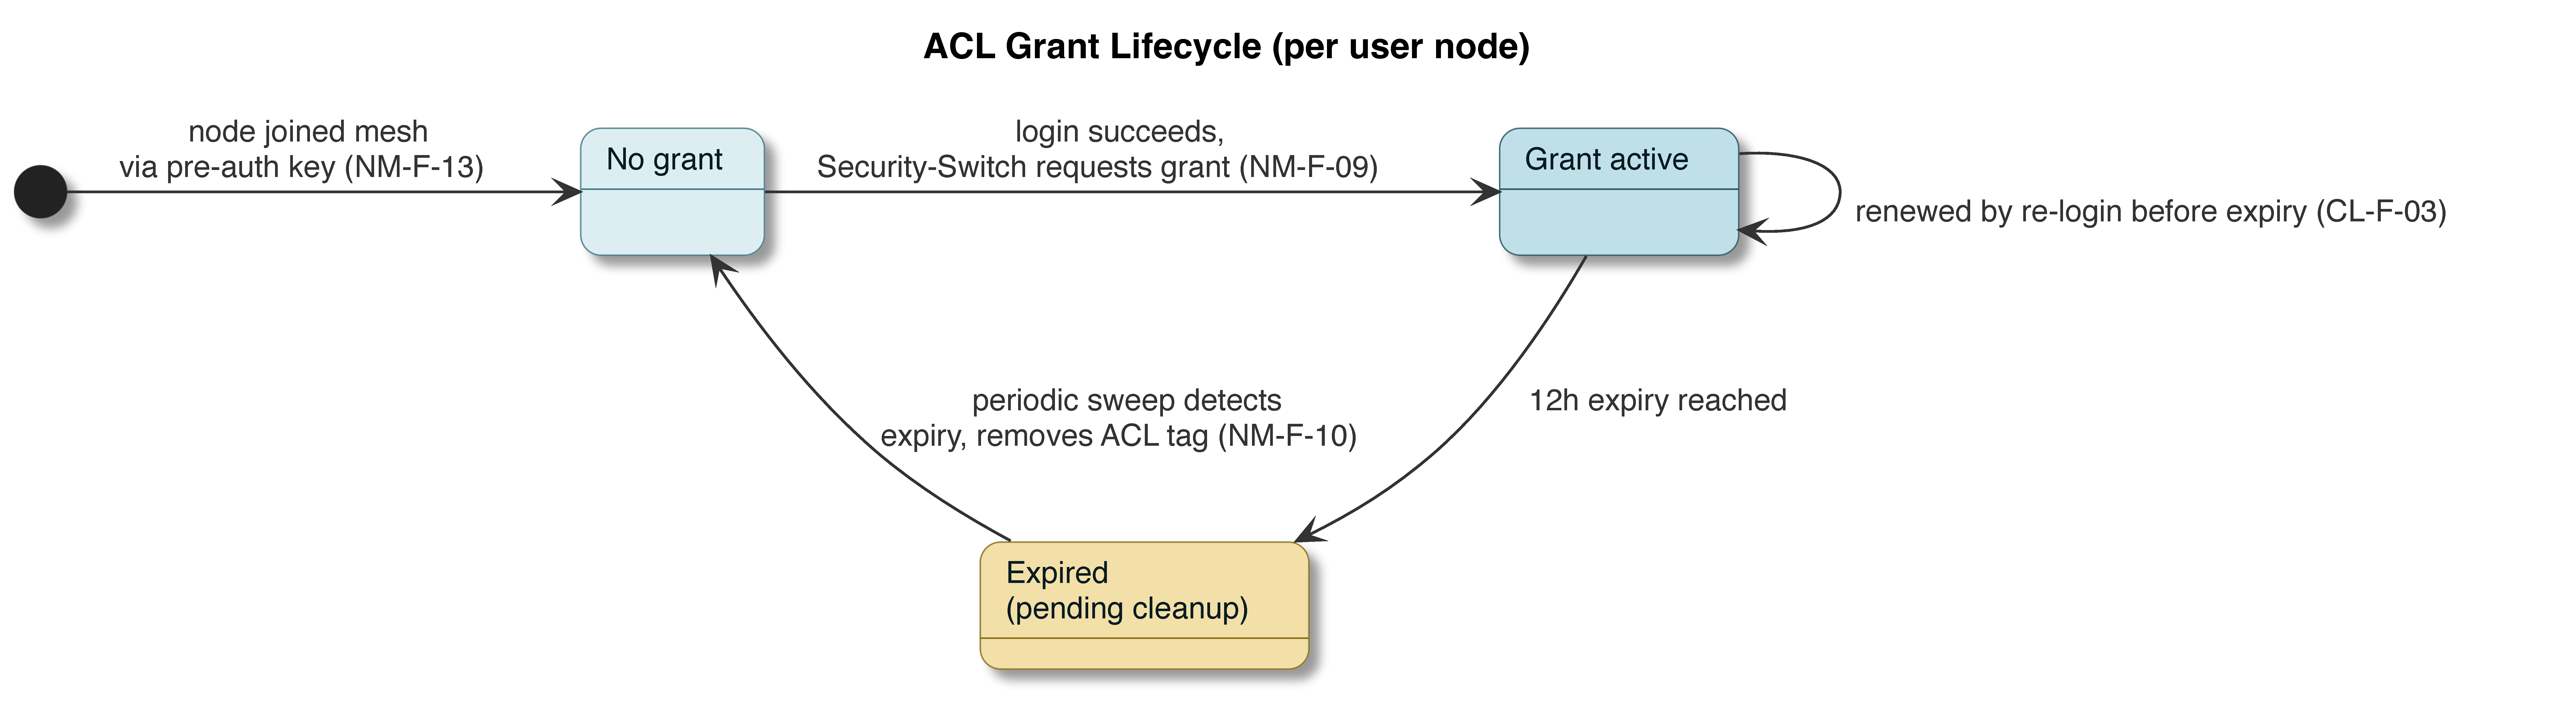
\includegraphics[width=\textwidth]{figures/10-operations-state-acl-grant.pdf}
    \caption{Ciclo di vita del permesso di accesso associato al nodo di un utente.}
    \label{fig:acl-grant}
\end{figure}


\section{Il paradosso del coordinatore: Headscale come servizio a sé}
\label{sec:paradosso-coordinatore}

La documentazione di Headscale dichiara che non è consigliato eseguire Headscale su una macchina che 
appartiene alla rete coordinata, perché può creare problemi alla risoluzione dei nomi tramite MagicDNS 
\cite{headscale-faq}. 

Il coordinatore deve perciò restare estraneo alla rete che coordina, e da qui discendono tre conseguenze.

La prima è che non può condividere una macchina virtuale o un container con nessun altro componente, 
perché tutti gli altri sono membri della mesh.

La seconda è che il traffico con cui Network-Manager crea le chiavi e assegna i tag non può essere
protetto dalla collocazione in rete, come invece accade per ogni altra chiamata interna. È l'unica
chiamata tra componenti del sistema che attraversa la rete pubblica, e l'unica la cui protezione dipende
interamente da mTLS.

La terza è che il coordinatore deve essere raggiungibile pubblicamente, perché un dispositivo che non è
ancora entrato nella rete deve poterlo contattare la prima volta per poter entrare nella rete.

Headscale ha però una limitazione rilevante per RAM-USB: non offre alcun modo di separare il protocollo di 
coordinamento, che deve essere raggiunto da tutti, dall'API amministrativa, che deve essere raggiunta solo da
Network-Manager. 
La separazione è stata affidata a un reverse proxy, che distingue le due superfici in base al percorso
della richiesta \cite{ramusb-code-headscale-proxy}. Le richieste di coordinamento passano senza alcun controllo,
mentre quelle amministrative sono accettate solo se accompagnate da un certificato emesso dalla 
Certificate-Authority privata, a cui si aggiunge anche una chiave API che Headscale richiede per conto 
proprio. Il traffico amministrativo è difeso da due credenziali indipendenti perché è una delle superfici 
più sensibili.

Il certificato presentato dal proxy è invece emesso da una CA pubblica, per la stessa ragione per cui lo
è quello di Entry-Hub. 

\section{CG-NAT e la necessità di un endpoint pubblico dedicato}

Visto che gli indirizzi IPv4 sono ormai terminati, gli Internet Service Providers assegnano ai router 
domestici dei clienti un IPv4 condiviso tra più clienti nel range \texttt{100.64.0.0/10} 
rendendo impossibile ai clienti esporre un proprio server su internet. Questo tipo di natting prende il nome
di Carrier-Grade NAT \cite{rfc6598}.
Visto che RAM-USB è progettato per essere hostato anche da utenti consumer, che potrebbero quindi non possedere
un IPv4 pubblico o un IPv6, Headscale ed Entry-Hub risiedono su un Virtual Private Server, separato dal 
resto del sistema. Il \autoref{chap:deployment} descrive la collocazione effettiva di ciascun componente.

\chapter{Osservabilità e metriche}
\label{chap:osservabilita}

\section{Pubblicazione delle metriche}

Le metriche operative possono tipicamente raggiungere chi le osserva in due modi: o è qualcun altro a 
interrogare periodicamente ogni servizio (\emph{pull}), oppure è ogni servizio a inviarle di propria 
iniziativa (\emph{push}). 
RAM-USB adotta il secondo: ogni servizio pubblica le proprie metriche una volta al minuto,
sul proprio topic MQTT dedicato verso il broker Mosquitto \cite{mosquitto-github}. 
La scelta deriva dal fatto che un modello \emph{pull} richiederebbe che Metrics-Collector apra una 
connessione verso ciascuno dei sei servizi, ampliando le regole di reachability della mesh discusse nel 
capitolo 7.
Pubblicando di propria iniziativa, sono invece i servizi ad aprire la connessione verso il broker.
Da lì, Metrics-Collector legge le metriche e le persiste in un database.

Le metriche operative non contengono dati degli utenti, ma i metadati del sistema vanno protetti con la 
stessa cura, per questo le comunicazioni avvengono all'interno della rete privata e protette dal mTLS, 
certificato dalla CA interna.

Ogni pubblicazione usa \emph{QoS 1}, (at least once) nella classificazione MQTT \cite{oasis-mqtt-311}: il
broker garantisce che il messaggio arrivi almeno una volta, al costo di un possibile duplicato. \emph{QoS 0},
(at most once), è escluso perché RAM-USB non può permettersi di perdere metriche in silenzio; \emph{QoS 2},
(exactly once), è escluso perché la garanzia in più che offre (l'assenza di duplicati) qui non serve
visto che un duplicato si traduce solo in due punti sovrapposti nello stesso istante, invisibili sul
grafico.

Ogni pubblicazione porta come corpo un payload di sei campi, riportato nel \autoref{lst:metrics-payload}.
I campi sono rispettivamente: l'identificativo del servizio che sta pubblicando, l'istante della 
pubblicazione, il numero di richieste gestite nell'ultimo minuto, il numero di errori rilevati nell'ultimo 
minuto, il tempo di risposta medio dell'ultimo minuto in millisecondi e il numero di connessioni che 
risultano aperte in quel momento. 

\Needspace{10\baselineskip}
\begin{lstlisting}[caption={Struttura del payload delle metriche, da \texttt{payload.go}
\cite{ramusb-code-metrics-payload}.}, label={lst:metrics-payload}]
type Payload struct {
	Service               string  `json:"service"`
	Timestamp             string  `json:"timestamp"`
	RequestCount          int64   `json:"request_count"`
	ErrorCount            int64   `json:"error_count"`
	AverageResponseTimeMs float64 `json:"average_response_time_ms"` 
	ActiveConnections     int64   `json:"active_connections"`
}
\end{lstlisting}

\section{Ricezione e controllo di coerenza}

Il messaggio pubblicato deve arrivare a un solo destinatario, e a nessun altro. Questa proprietà è garantita 
dall'ACL di Mosquitto che garantisce che ogni servizio possa solo scrivere sul proprio topic, mentre 
Metrics-Collector può leggere dai topic \texttt{metrics/\#} senza potervi scrivere.

Quell'ACL, però, non impedisce che un servizio compromesso, pur restando entro il proprio permesso di 
scrittura legittimo, pubblichi un payload il cui campo \texttt{service} dichiarato sia un nome diverso dal 
proprio.
Metrics-Collector rivalida quindi ogni messaggio in modo indipendente, derivando il servizio
atteso dal topic di arrivo e confrontandolo con quello dichiarato nel payload. 
Su qualunque discrepanza scarta il messaggio e lo registra nei log.

\section{Persistenza delle serie temporali}

Metrics-Collector persiste le metriche in TimescaleDB \cite{timescaledb-github}, un'estensione di 
PostgreSQL pensata per un carico fatto quasi solo di scritture ordinate nel tempo. 

La tabella \texttt{metrics} non ha una chiave primaria dato che una riga di metriche non ha un'identità 
naturale, inoltre, TimescaleDB \cite{timescaledb-github} non ne richiede una. È organizzata in chunk per
intervalli di tempo sulla colonna \texttt{time}: le due politiche in background del
\autoref{lst:metrics-policies} agiscono chunk per chunk, in base alla loro età. La prima elimina ogni chunk
più vecchio di trenta giorni; la seconda, dopo sette giorni, sposta i chunk in un formato compresso a
colonne, raggruppato per servizio e ordinato per tempo decrescente.

\Needspace{18\baselineskip}
\begin{lstlisting}[language=sql, caption={Politiche automatiche di ritenzione e compressione della tabella
\texttt{metrics}, da \texttt{000001\_create\_metrics\_table.up.sql} \cite{ramusb-code-metrics-schema}.},
label={lst:metrics-policies}]
SELECT create_hypertable('metrics', by_range('time'));

SELECT add_retention_policy('metrics', drop_after => INTERVAL '30 days');

ALTER TABLE metrics SET (
	timescaledb.enable_columnstore,
	timescaledb.segmentby = 'service',
	timescaledb.orderby = 'time DESC'
);
CALL add_columnstore_policy('metrics', after => INTERVAL '7 days');
\end{lstlisting}

\section{Visualizzazione delle metriche}

Un amministratore consulta lo stato di salute del sistema, senza che quella consultazione 
tocchi mai i dati degli utenti visto che per costruzione, le metriche non ne contengono. 
Grafana \cite{grafana-github} legge da TimescaleDB direttamente.

Per contattare TimescaleDB, oltre alla raggiungibilità sulla rete mesh e al certificato mTLS di Grafana, 
è richiesta anche una password, sullo stesso principio di difesa in profondità già visto per l'API 
amministrativa di Headscale nel capitolo 7.

La dashboard mostra tre pannelli, ciascuno una query diretta sulla tabella \texttt{metrics}: tempo medio di
risposta, throughput e connessioni attive. 

La \autoref{fig:metrics-flow} riassume l'intera pipeline appena descritta, dalla pubblicazione sul topic
MQTT alla dashboard.

\begin{figure}[H]
    \centering
    \includegraphics[width=\textwidth]{figures/11-operations-metrics-flow.pdf}
    \caption{Pipeline di osservabilità, dalla pubblicazione delle metriche alla dashboard di Grafana.}
    \label{fig:metrics-flow}
\end{figure}

\chapter{Testing e validazione}

\section{Il modello V e i quattro livelli di test}
%% TODO: unit/component, integration (UC-01..05), system (RNF-*), acceptance (RU-*) — legati alla granularità della specifica, non alla fase di progetto.

\section{Strategia di integrazione bottom-up}
%% TODO: perché si parte da Database-Vault (meno dipendenze uscenti, più requisiti concentrati DV-F-01..20), driver/stub scritti a mano.

\section{TDD: criteri di ingresso e uscita}
%% TODO: test scritto e fallito prima dell'implementazione, decision coverage sulle funzioni di validazione, tracciabilità bidirezionale via doc comment.

\section{Copertura e lacune del piano di test}
%% TODO: cosa il Test Plan dichiara non coperto (load/stress testing rimandato, nessun test per RISK-01/02) — solo lacune di test, i rischi di progetto più ampi restano nel cap. 11.

\chapter{Deployment}

\section{Containerizzazione: build multi-stage e supervisione s6-overlay}
%% TODO: pattern comune a più servizi, processi multipli supervisionati nello stesso container (es. tailscaled reale + binario Go).

\section{Docker locale vs Proxmox VE: due livelli di isolamento}
%% TODO: perché non sono alternativi (Docker per portabilità/isolamento per-servizio, Proxmox per isolamento più forte e HA potenziale), KVM per Storage-Service/Database-Vault/Network-Manager vs LXC per gli altri (RNF-ORG-04).

\section{Topologia distribuita: un Compose file per servizio}
%% TODO: perché non un unico file merged, ma tanti quanti i servizi, per rispecchiare la reale distribuzione su VM/host Proxmox separati.

\chapter{Analisi critica delle proprietà di sicurezza}
\label{chap:sicurezza}

\section{Scenari di attacco e mitigazioni}
%% TODO: walkthrough concreto dal punto di vista dell'attaccante — compromissione isolata di un componente, credenziali rubate, tentativo di replay di una pre-auth key, richiesta falsificata a un servizio interno — e come le difese già descritte nei cap. 4-8 rispondono a ciascuno scenario. Esempi concreti di requisiti non funzionali imposti a livello di tipo, non di convenzione: pkg/errors lega un costruttore al codice HTTP, garantendo che il messaggio pubblico sia sempre quello sanitizzato (impossibile far trapelare un dettaglio interno per errore); pkg/logging tipizza i campi email/password come un tipo dedicato che implementa slog.LogValuer e stampa sempre REDACTED — DV-F-03/RD-01 (niente credenziali nei log) garantito dal type system, non dalla disciplina del singolo sviluppatore.
%% TODO: enumerazione delle email registrate — POST /api/users risponde 201 se l'email era libera e 409 se esisteva già (DV-F-12), quindi un utente esterno non autenticato può testarne una alla volta; contrasto esplicito con DV-F-15, che al login collassa "email inesistente" e "password errata" nello stesso 401 proprio per impedire questa deduzione, protezione mai estesa alla registrazione. Effetto collaterale: una sonda "riuscita" (201) registra davvero l'account sull'email sondata, che EH-F-04 valida solo nel formato e non come posseduta (nessun link di conferma), rendendola per sempre non registrabile dal legittimo proprietario (nessun path di cancellazione). Promessa fatta al lettore in 4.1.3; tracciata come KI-106 in docs/Known_Issues.md, non presente tra i rischi accettati della SRS sezione 8.
%% TODO: accesso amministrativo alle credenziali — RNF-SEC-01 ammette che email e password transitano attraverso Entry-Hub, Security-Switch e Database-Vault per validazione e hashing (cifrate in TLS/mTLS, mai persistite né loggate in chiaro): chi controlla uno di quei tre processi può leggerle nel punto in cui sono in chiaro in memoria. A riposo il quadro è diverso: la password non è recuperabile (Argon2id, DV-F-07), mentre l'email lo è per chi possiede la master key (DV-F-04/DV-F-05, chiave in variabile d'ambiente, RISK-02). Distinguere i due piani (in transito e a riposo) e dire cosa comporta per RU-06. Promessa fatta al lettore in 4.1.3.

%% TODO: verifica offline di un indirizzo a partire da una copia del database (RISK-06). Distinguerlo dai due casi sopra costruendo la scala di cosa serve all'attaccante: l'enumerazione via 409 richiede solo accesso di rete all'API e nessun dato; questa richiede il dump ma nessuna chiave, perche' la chiave di ricerca e' uno SHA-256 senza chiave e basta ricalcolarlo su un indirizzo candidato; la decifratura dell'email richiede dump piu' master key. Precisare il limite senza sopravvalutarlo: non si invertono gli hash, si testano candidati, ma un dizionario di indirizzi comuni copre gia' molto, quindi "non puo' ricavare gli indirizzi che non sospetta" e' vero in senso stretto e debole in pratica. La mitigazione (chiave di ricerca via HMAC sotto il pepper) sta negli sviluppi futuri del cap. 12.

\section{Isolamento dei fallimenti}
%% TODO: perché la compromissione di un componente non si propaga agli altri, sintesi di trust zones (cap. 4) + mTLS + ri-validazione indipendente (cap. 3/5) + isolamento a livello di deployment (container/Proxmox, cap. 10), vista dalla lente "cosa succede se X viene compromesso" — non ripetere l'elenco dei limiti noti, quello resta nel cap. 12.

\section{Costo delle scelte architetturali}
%% TODO: tabella di sintesi a tre colonne — scelta architetturale, proprietà che garantisce, prezzo pagato — che raccoglie i costi già pagati nei capitoli di meccanismo invece di introdurne di nuovi: separazione in quattro processi (rivalidazione indipendente e isolamento dei fallimenti, contro latenza per hop e nessuno strato saltabile, sezione 4.2), mTLS su ogni comunicazione interna (autenticazione reciproca, contro un certificato per componente da emettere e rinnovare, sezione 4.4), CA privata unica (fiducia verificabile end-to-end, contro punto singolo di fiducia, sottosezione 4.1.6), rete mesh come confine di raggiungibilità (Storage-Service invisibile ai non autenticati, contro dipendenza dal coordinatore e RISK-04, cap. 7), Argon2id con parametri alti (resistenza al brute force offline, contro memoria e latenza per ogni login, cap. 5), backup su filesystem via SFTP invece che a blocchi (isolamento chroot come oggetto di studio, contro la complessità di ST-F-06..ST-F-11, cap. 6). Ogni riga rimanda al capitolo che la discute: qui si somma il conto, non si ripete l'argomento.

\chapter{Conclusioni}
\label{chap:conclusioni}

\section{Risultati raggiunti}

Il \autoref{chap:introduzione} affida a RAM-USB l'obiettivo di progettare, implementare e validare un
servizio di backup remoto multi-utente rispetto ai requisiti della SRS \cite{ramusb-srs}, affidandosi ai
principi zero-trust e defense-in-depth per difendere il sistema da attacchi esterni, non per competere
con le soluzioni commerciali esistenti ma per discuterne le scelte di design in modo trasparente.

I dieci requisiti utente elencati nel \autoref{chap:requisiti} sono, con una sola eccezione, coperti da requisiti di
sistema implementati e tracciati fino al codice. Un utente può registrarsi fornendo solo email, password
e chiave pubblica SSH (RU-01), autenticarsi nelle sessioni successive (RU-02), caricare e recuperare
backup cifrati lato client da qualunque luogo (RU-03, RU-07), farlo solo dopo essersi autenticato (RU-04),
con la garanzia che né la password né il contenuto dei backup siano mai leggibili da un amministratore
(RU-05, RU-06), in uno spazio isolato da quello degli altri utenti (RU-08). Un amministratore può
osservare la salute e le prestazioni del sistema senza mai toccare i dati dei singoli utenti (RU-10).

L'unica eccezione è RU-09, la garanzia che nessuno possa modificare o cancellare un backup: è stata
dichiarata fuori perimetro fin dalla SRS, per i tempi stretti del progetto piuttosto che per una scelta di
design, ed è ripresa nella prossima sezione.

Le cinque sequenze d'uso che attraversano il sistema, registrazione, login, backup, restore e
consultazione delle metriche, non sono rimaste un esercizio sulla carta: sono state eseguite end-to-end
sul deployment reale su Proxmox, non solo sullo stack Docker di sviluppo, con gli stessi risultati
riportati nel \autoref{chap:testing}.

\section{Limiti noti}

La SRS accetta esplicitamente quattro rischi come costo del rilascio nei tempi previsti, non come
sviste \cite{ramusb-srs}. Dichiararli qui, uno per uno, è la stessa disciplina di onestà già applicata nel
\autoref{chap:sicurezza}, dove ogni proprietà che regge viene dichiarata insieme a quella che cade.

RISK-01 è RU-09 stesso: nessun requisito di sistema impedisce a un amministratore di modificare o
cancellare un backup. Resta un miglioramento desiderabile, non ancora costruito.

RISK-02 riguarda la master key: risiede in una variabile d'ambiente, senza una procedura di backup
(DV-F-18) né di rotazione (DV-F-19), entrambe requisiti "dovrebbe" e non "deve". La sua perdita
comporterebbe la perdita irreversibile dell'accesso a tutti i dati cifrati; la sua compromissione
romperebbe la garanzia zero-knowledge per ogni utente.

RISK-03 riguarda il client, pensato per girare nativamente sulla macchina dell'utente e non come
container Docker. Containerizzarlo è stato considerato e scartato per ora: un container non vede percorsi
arbitrari dell'host, come il Desktop dell'utente, a meno di un bind mount esplicito, e l'insieme dei file
da salvare si sceglie liberamente al momento del backup, non è noto in anticipo come per ogni altro
componente. L'opzione che perde meno isolamento, se il tema fosse ripreso, è un bind mount per singola
invocazione, limitato alla sola cartella oggetto del backup.

RISK-04 è la dipendenza circolare della risoluzione DNS di Network-Manager dal proprio stesso MagicDNS: se
Network-Manager pubblicasse una policy ACL non funzionante, potrebbe perdere anche la capacità di
risolvere l'hostname di Headscale di cui avrebbe bisogno per correggerla. La scelta di accettare comunque
il MagicDNS, invece di costruire un percorso di recupero automatico, è un rischio accettato per scelta
esplicita, non un difetto scoperto in seguito: in questo scenario di guasto, un operatore interviene
manualmente.

\section{Sviluppi futuri}

\subsection{Mitigazione dell'enumerazione degli indirizzi email}

Il \autoref{sec:scenari-attacco} analizza RISK-05: la registrazione rivela, tramite il codice HTTP
restituito, se un indirizzo è già registrato. Il comportamento ideale risponderebbe in modo identico in
entrambi i casi, per esempio sempre con un 202, mentre l'esito reale viaggerebbe fuori banda, in un'email
di conferma inviata all'indirizzo indicato: solo chi possiede davvero quella casella riceverebbe il
seguito, mentre chi sonda l'endpoint riceverebbe sempre la stessa risposta. Un effetto collaterale
positivo scomparirebbe insieme al problema: senza un account attivato dalla conferma, sparirebbe anche
l'occupazione abusiva di un indirizzo altrui.

Il costo non va taciuto: servirebbe una capacità di invio email che il sistema oggi non ha,
un client SMTP, token di conferma con scadenza, e una deliverability affidabile. Cambierebbe inoltre
UC-01, perché la pre-auth key oggi viaggia dentro la risposta 201 della registrazione, mentre con una
registrazione in due tempi dovrebbe essere consegnata solo dopo la conferma.

\subsection{Le due regole della policy delle password}

Il \autoref{sec:entropia} misura che, sotto scelta uniforme, il vincolo di almeno tre categorie di
carattere vale meno di un decimo di bit di entropia, mentre un carattere aggiuntivo ne vale 6,57: sotto
quell'ipotesi la regola di composizione è ridondante per costruzione, perché una password davvero casuale
usa già più categorie da sé. Il suo scopo reale, però, non è aumentare l'entropia, ma vincolare la scelta
di una persona, e lì il suo valore non è misurabile senza la distribuzione reale delle password scelte
dagli utenti.

Restano due direzioni da confrontare: tenere entrambe le regole così come sono, oppure eliminare il
vincolo di composizione e alzare la lunghezza minima, la strada indicata dalle linee guida NIST correnti
\cite{nist-sp-800-63b}, che raccomandano ai verificatori di non imporre regole di composizione e portano
il minimo per una password usata da sola a 15 caratteri. Anche la seconda strada ha però un costo da non
nascondere: senza una lista di password compromesse note, togliere il vincolo di composizione rimuove
una protezione debole senza sostituirla con una forte, e una password come \texttt{password} tornerebbe
accettabile.

\subsection{Hash con chiave per la ricerca dell'email}

Il \autoref{sec:scenari-attacco} analizza anche RISK-06: la chiave di ricerca dell'email è oggi uno
SHA-256 senza chiave, veloce da calcolare su uno spazio di indirizzi piccolo e indovinabile. Il
comportamento ideale deriverebbe quella chiave con una funzione dotata di chiave, HMAC-SHA256 sotto il
pepper, e non con la concatenazione ingenua che nel percorso della password basta solo perché lì
interviene Argon2id. Un pepper è compatibile con la ricerca, a differenza di un salt: essendo un unico
segreto globale, il digest resta deterministico e la ricerca al login continua a funzionare identica. Il
guadagno sarebbe che una copia del database, da sola, non permetterebbe più di verificare se un indirizzo
sia registrato, la stessa protezione che Argon2id offre già per la password. Non
risolverebbe invece RISK-05, che resta un attacco online contro l'API: sono due superfici diverse.

Il costo dichiarato dalla SRS per questa modifica presuppone però una reversibilità che oggi non esiste
ancora nel codice, e va corretto qui. La SRS descrive ogni \texttt{email\_hash} come ricostruibile
decifrando l'email con la master key, dato che è cifrata e non solo hashata; il record salvato, insieme
alla master key, contiene sì in linea di principio tutto il necessario.

\texttt{encryption.go}, però, dichiara oggi solo \texttt{EncryptEmail}, non la funzione inversa: nessun
percorso del codice decifra mai quella colonna. La reversibilità è quindi, per ora, una proprietà dei dati
salvati, non ancora del sistema: la migrazione dovrebbe prima scrivere quel percorso di decifratura
mancante, non solo invalidare e ricalcolare gli hash esistenti.

Il costo resta comunque reale anche a percorso scritto: il pepper diventerebbe portante anche per la
ricerca dei record, non solo per la verifica delle password, spostando la conseguenza della sua perdita da
"non si verificano più le password" a "non si trovano più i record", da valutare accanto a RISK-02.

\subsection{Altri requisiti "dovrebbe" non implementati}

Oltre a DV-F-18 e DV-F-19, già discussi come RISK-02, restano "dovrebbe" e non ancora costruiti il limite
di quota per utente (ST-F-14) e la replica automatica dei backup su CephFS (ST-F-15), entrambi rimandati
nella SRS come miglioramenti desiderabili piuttosto che vincoli del progetto. Resta inoltre da fare, sul
piano della verifica piuttosto che dell'implementazione, un test di carico e di stress che misuri il
sistema oltre le condizioni già esercitate in questa tesi.


%% Fine dei capitoli normali, inizio dei capitoli-appendice (opzionali)
\appendix

%\part{Appendici}

%% Appendici: un file per appendice sotto appendices/, richiamato con \input.
\chapter{Titolo della prima appendice}
Sed purus libero, vestibulum ut nibh vitae, mollis ultricies augue. Pellentesque velit libero, tempor sed pulvinar non, fermentum eu leo. Duis posuere eleifend nulla eget sagittis. Nam laoreet accumsan rutrum. Interdum et malesuada fames ac ante ipsum primis in faucibus. Curabitur eget libero quis leo porttitor vehicula eget nec odio. Proin euismod interdum ligula non ultricies. Maecenas sit amet accumsan sapien.


%% Parte conclusiva del documento; tipicamente per riassunto, bibliografia e/o indice analitico.
\backmatter

%% Riassunto (opzionale)
%\summary
%Maecenas tempor elit sed arcu commodo, dapibus sagittis leo egestas. Praesent at ultrices urna. Integer et nibh in augue mollis facilisis sit amet eget magna. Fusce at porttitor sapien. Phasellus imperdiet, felis et molestie vulputate, mauris sapien tincidunt justo, in lacinia velit nisi nec ipsum. Duis elementum pharetra lorem, ut pellentesque nulla congue et. Sed eu venenatis tellus, pharetra cursus felis. Sed et luctus nunc. Aenean commodo, neque a aliquam bibendum, mauris augue fringilla justo, et scelerisque odio mi sit amet diam. Nulla at placerat nibh, nec rutrum urna. Donec ut egestas magna. Aliquam erat volutpat. Phasellus vestibulum justo sed purus mattis, vitae lacinia magna viverra. Nulla rutrum diam dui, vel semper mi mattis ac. Vestibulum ante ipsum primis in faucibus orci luctus et ultrices posuere cubilia Curae; Donec id vestibulum lectus, eget tristique est.

%% Bibliografia (praticamente obbligatoria)
\bibliographystyle{plain_\languagename}%% Carica l'omonimo file .bst, dove \languagename è la lingua attiva.
%% Nel caso in cui si usi un file .bib (consigliato)
\bibliography{thud}
%% Nel caso di bibliografia manuale, usare l'environment thebibliography.

%% Per l'indice analitico, usare il pacchetto makeidx (o analogo).

\end{document}

--- Istruzioni per l'aggiunta di nuove lingue ---
Per ogni nuova lingua utilizzata aggiungere nel preambolo il seguente spezzone:
    \addto\captionsitalian{%
        \def\abstractname{Sommario}%
        \def\acknowledgementsname{Ringraziamenti}%
        \def\authorcontactsname{Contatti dell'autore}%
        \def\candidatename{Candidato}%
        \def\chairname{Direttore}%
        \def\conclusionsname{Conclusioni}%
        \def\cosupervisorname{Co-relatore}%
        \def\cosupervisorsname{Co-relatori}%
        \def\cyclename{Ciclo}%
        \def\datename{Anno accademico}%
        \def\indexname{Indice analitico}%
        \def\institutecontactsname{Contatti dell'Istituto}%
        \def\introductionname{Introduzione}%
        \def\prefacename{Prefazione}%
        \def\reviewername{Controrelatore}%
        \def\reviewersname{Controrelatori}%
        %% Anno accademico
        \def\shortdatename{A.A.}%
        \def\summaryname{Riassunto}%
        \def\supervisorname{Relatore}%
        \def\supervisorsname{Relatori}%
        \def\thesisname{Tesi di \expandafter\ifcase\csname thud@target\endcsname Laurea\or Laurea Magistrale\or Dottorato\fi}%
        \def\tutorname{Tutor aziendale}%
        \def\tutorsname{Tutor aziendali}%
    }
sostituendo a "italian" (nella 1a riga) il nome della lingua e traducendo le varie voci.

